\chapter{Experiments}
\label{chapter:experiments}

We use 25 benchmark problems from the CEC 2005 Special Session on Real-Parameter Optimization to test the performance of our new techniques.
The CEC 2005 benchmark problems are composed of both standard test problems \textit{e.g.} Sphere, Schwefel's, Rosenbrock's, Rastrigin's, etc.,
and some hybrid problems.
We tested the CMA-ES, PSO, and ACO$_R$ algorithms with and without our new techniques.
The results show that our technique reduces the average error of CMA-ES and ACO$_R$ on some multimodal problems.  

\section{CEC 2005 Benchmark Problems}

The special session on real-paramter optimization of CEC 2005~\cite{Suganthan:2005:benchmark} aims to evaluate different algorithms in a more systematic manner by specifying a common termination criterion, size of problems, linkages/rotation, etc.
It consists of 25 minimization problems with $2, 10, 30, 50$ dimensions.
The evaluation requires 25 runs, each with maximum evaluations $10000 * D$. 
Initialization is required to be uniform random within the search space, except for problems 7 and 25, for which initialization ranges are specified.
Similarly, the global optimum exists within the given bounds, except for problem 7 and 25.
The algorithm is terminated one it reaches the maximum evaluations or if the minimum error in the function value is less than $10^{-8}$.
Here we only tested on the 2-dimensional problems, 
since our technique consumes too much time on higher dimensions, 
making optimization impractical.  
Also, we modified the Problem 11 and 12 by adding the Euclidean distance to the bias position in the fitness function,
so that there exists only one global optimum solution in the search space.
Further speedup and studies to expend the technique on higher dimension are needed.
We show the average and median error plots for all 25 problems in the following section.
%The tables, following the requested format in~\cite{Suganthan:2005:benchmark}, are also given the the following section.  


\section{Experiment Settings}

In this section, we briefly describe the parameters setting for CMA-ES, SPSO and ACOR.

We use the \textit{Covariance Matrix Adaptation Evolution Strategy for non-linear numerical optimization in Python} package~\footnote{https://pypi.python.org/pypi/cma} provided by Hensen, the author of CMA-ES.
Although the default population for CMA-ES in $D$-dimension is set to be $4 + \lfloor3\log(D)\rfloor$, meaning default population size is 6 in 2D,
we found out that we a larger population for the MDL to not merge every particles into one cluster.
Therefore, we set the population size as 30 for CMA-ES.
The initial mean is set to be the center between max bounds and min bounds in every dimension.
The initial step-size is set to be one sixth of the maximum length between max bounds and min bounds in each dimension. 
It is suggested to let the global optimum be within three standard deviation~\cite{Hansen:2006:CMA_ES_review}.

As for the SPSO 2011, there are currently no official Python implementation, 
so we created our own Python implementation according to the tutorials~\cite{Clerc:2012:SPSO2011},
and the official SPSO 2011 C++ code provided by Clerc, the author of SPSO~\footnote{https://www.particleswarm.info}.
The population size is set to be 40 as suggested in~\cite{Clerc:2012:SPSO2011}.
The parameters $c = \frac{1}{2} + \ln(2) \simeq 1.193$ and $w = \frac{1}{2\ln(2)} \simeq 0.721$ are also set as default.
We implement the random topology with $K = 3$,
and update the topology at the beginning and in every iteration when the best fitness does not improve.
Also, we use the ``bounce back'' boundary condition suggested in~\cite{Clerc:2012:SPSO2011}, which is also described in Chapter~\ref{chapter:algos}.

For ACOR, we set our parameters according to the original paper~\cite{Socha:2008:ACOR}. 
The parameters are shown in Table~\ref{table:ACOR_parameters}.

\begin{table}%[t!]
\centering
\label{table:ACOR_parameters}
\begin{tabular}{lll}
\hline
Parameter                        & Symbol   & Value          \\ \hline
No. of ants used in an iteration & $m$      & $2$            \\
Speed of convergence             & $\xi$    & $0.85$         \\
Locality of the search process   & $q$      & $10^{-4}$      \\
Archive size                     & $k$      & $50$           \\ \hline
\end{tabular}
\caption{Summary of the parameters used by $ACO_R$}
\end{table}

%Describe our bandit parameters setting, including the initial population, maximum number of arms, and (1+1)-ES step size.

\section{Experiment Results}

Generally speaking, we can see a huge improvement in multimodal problems and hybrid problems
when combining our technique with ACO$_R$,
since the underlying model for ACO$_R$ is a Gaussian Kernel that intrinsically models hills.
We can see improvement in some cases when combining our technique with CMA-ES.
However, for SPSO, most of the results costs more evaluations to get to same error level.
This is because the underlying model for SPSO is not a Gaussian, but a random topology.
The flying particles make reclustering and redefining ROIs really unstable.


Problems 1 to 5 are unimodal functions.
The optimum solution of Problem 5 is on the diagonal of the search space, 
making it extremely easy to solve for SPSO and ACO$_R$.
Thus there is no error line for these two algorithms on Problem 5
We can see that CMA-ES is extremely efficient on solving unimodal problems, 
since the underlying model is a multivariate Gaussian and it converges very fast.
As expected, our methods to cost slightly more evaluations than the original algorithms on unimodal functions,
since we sample more points in the beginning. 
Also, although our clustering methods recognize unimodals in most of the times,
it is not good at handling narrow valleys, \textit{e.g.} Problem 3, 
and starts to split into multiple clusters once falls into the valley with small gradient.
This multiplication gets worse since the smaller the ROI becomes, the less gradient info there is.
Thus, the clustering methods would try its best to generate ``hills'' from the plane with almost no gradient.
This is the reason why our technique does not improve the original algorithms.
it falls into the valley


Problems 6 to 12 are basic multimodal functions.
We can see significant improvement in Problem 11 and Problem 12 on algorithm CMA-ES and ACO$_R$.
Besides, ACO$_R$ combined with our techniques leads with the minimum error in most of the problems.
This means that the divide-and-conquer technique works well on problems with multiple hills.
The narrow valley characteristics also appears in Problem 6, so we spend more evaluations than the original algorithms.
One interesting thing happens in Problem 9, where our technique failed to improve CMA-ES on a Rastrigin Problem.
We suspect that it is due not being able to recognize the small hills, since CMA-ES samples with a normal distribution.
Therefore, even if particles did get to the top of different hills, the MDL method would still recognize them as one normal distribution.
Thus, no reclustering was performed and the population converged to the wrong hills sometimes.

Problem 13 and Problem 14 are expended problems, and they are a bit too difficult for most of the algorithms.

Problems 15 to 25 are hybrid composition functions.
SPSO is suitable for these kinds of problems, since SPSO is good at exploring and takes a bit longer to converge.
However, our methods enhanced the ability of ACO$_R$, making it compatible with SPSO, and even better sometimes.



\begin{figure}
\centering
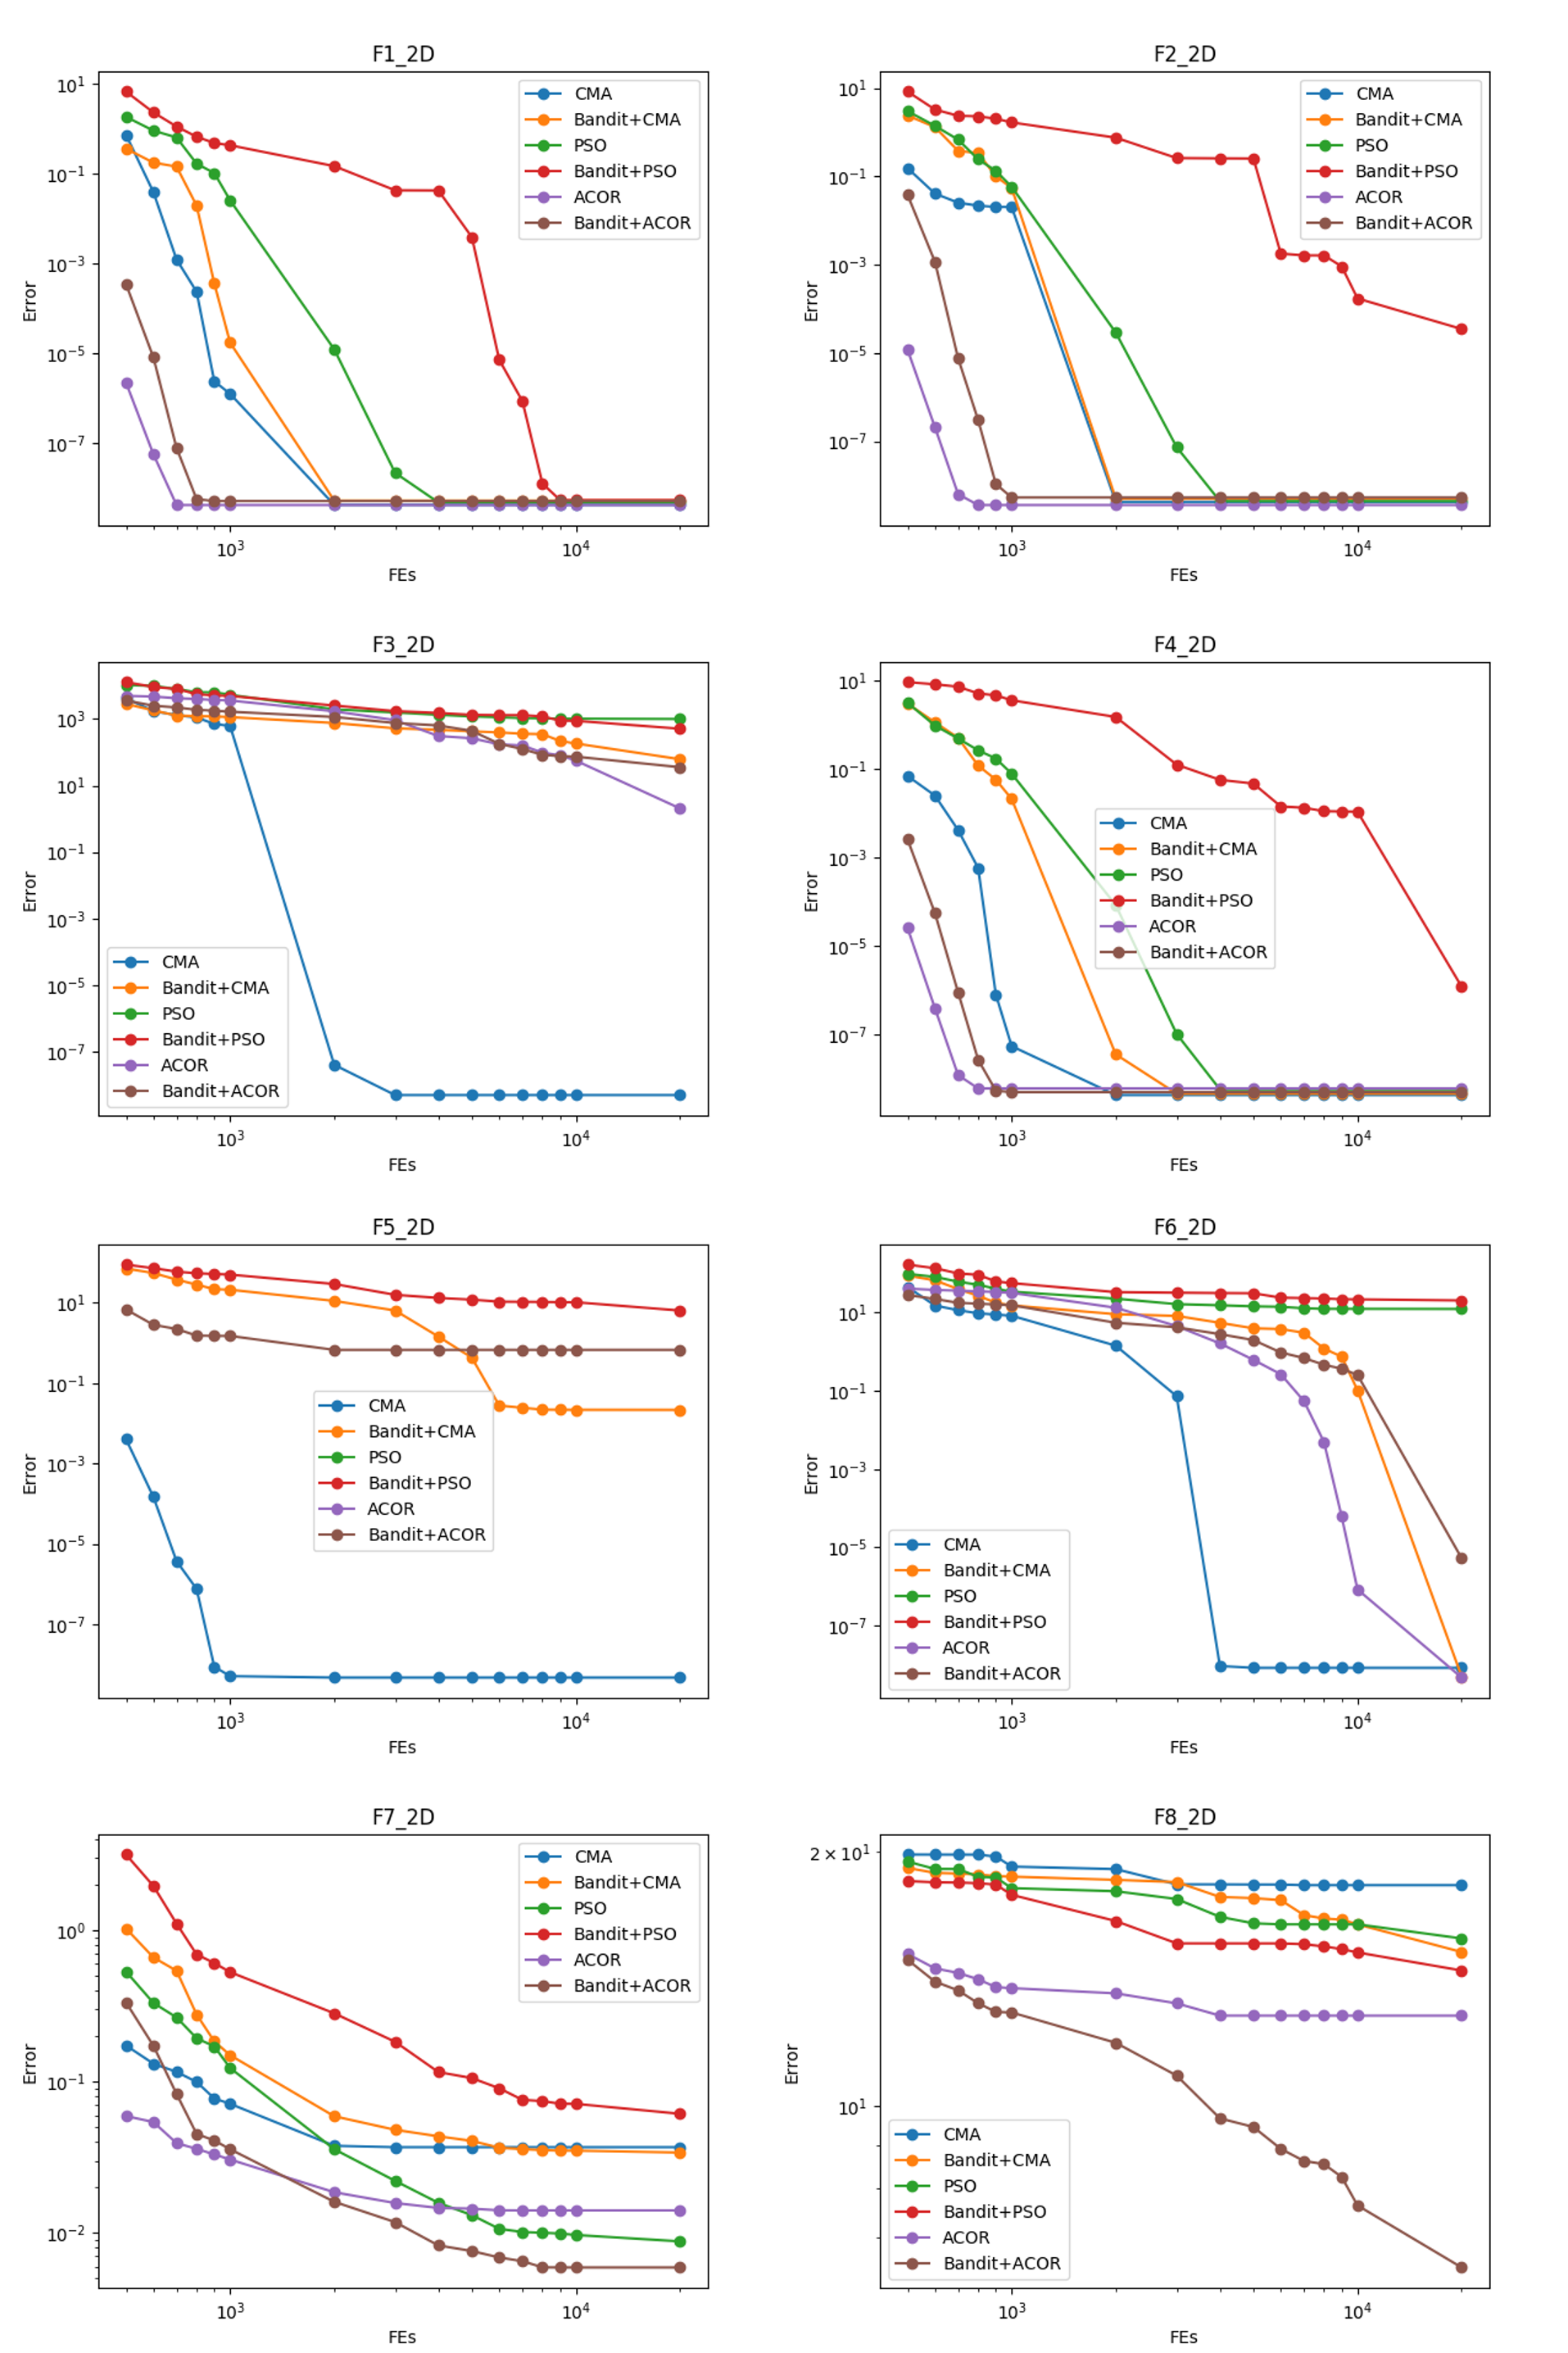
\includegraphics[width=\textwidth]{Average_F1_F8}
\caption{Average error of Problem 1 to Problem 8.}\label{fig:Average_F1_F8}
\end{figure}

\begin{figure}
\centering
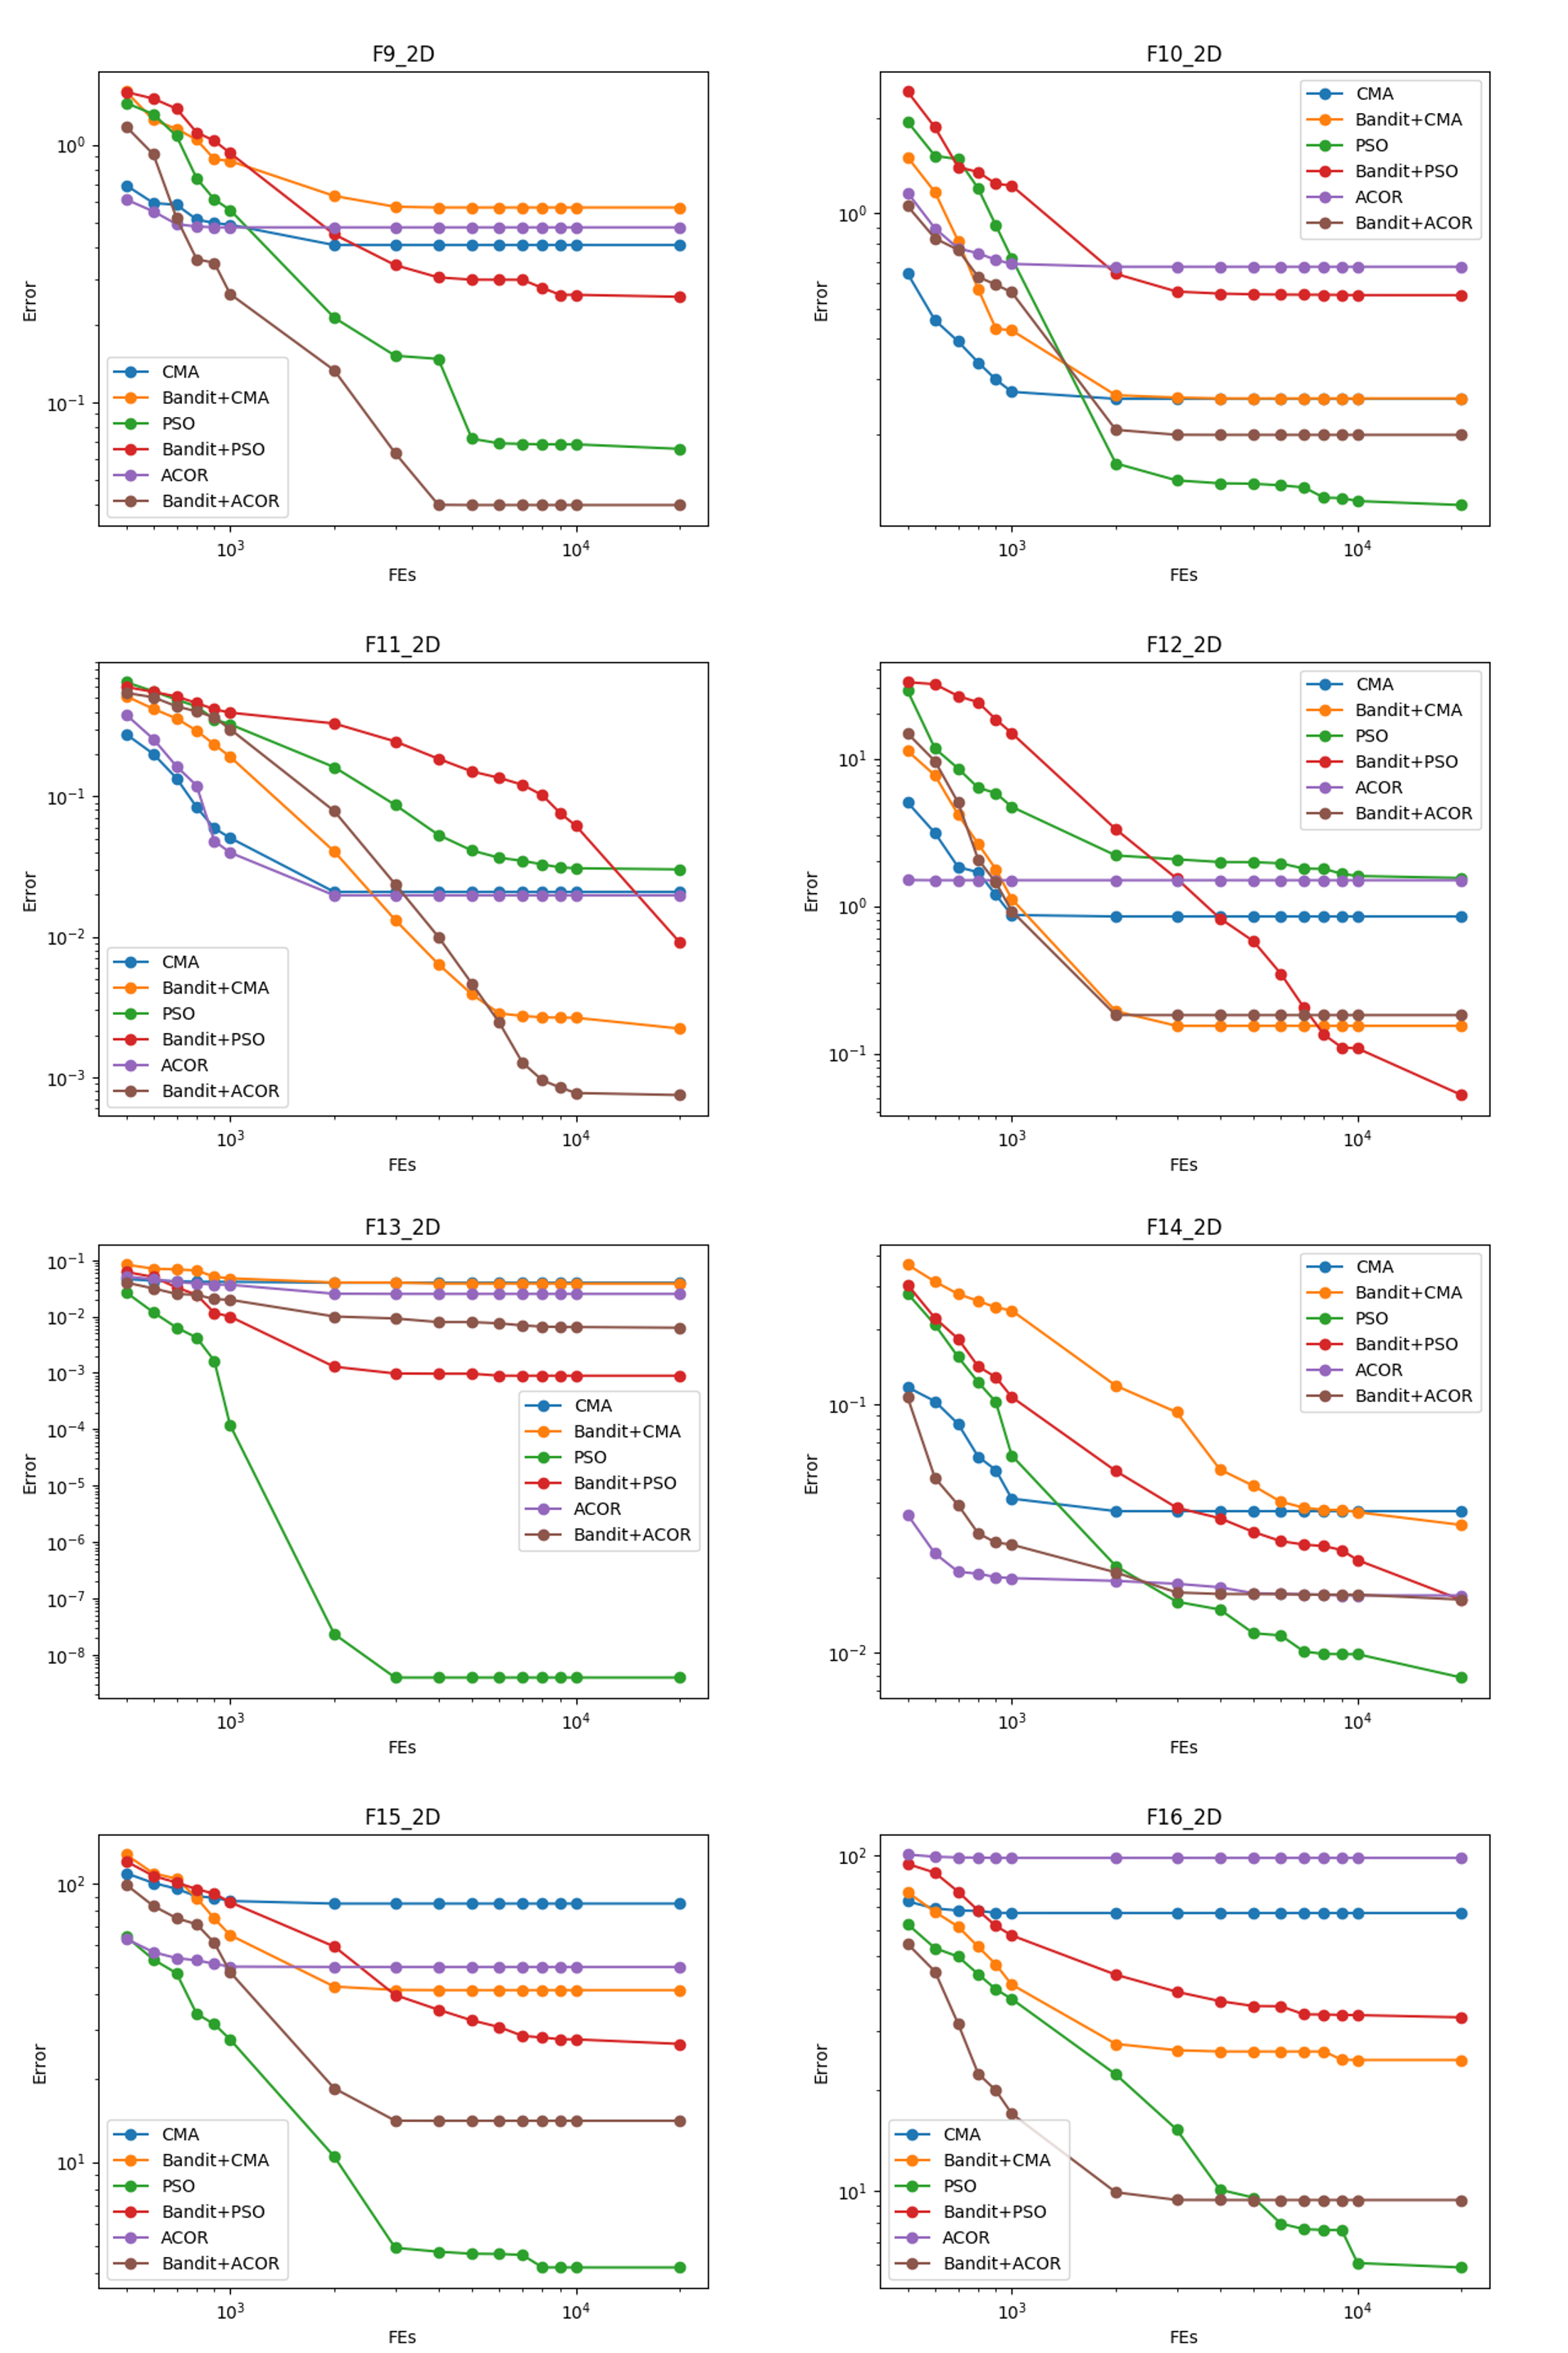
\includegraphics[width=\textwidth]{Average_F9_F16}
\caption{Average error of Problem 9 to Problem 16.}\label{fig:Average_F9_F16}
\end{figure}

\begin{figure}
\centering
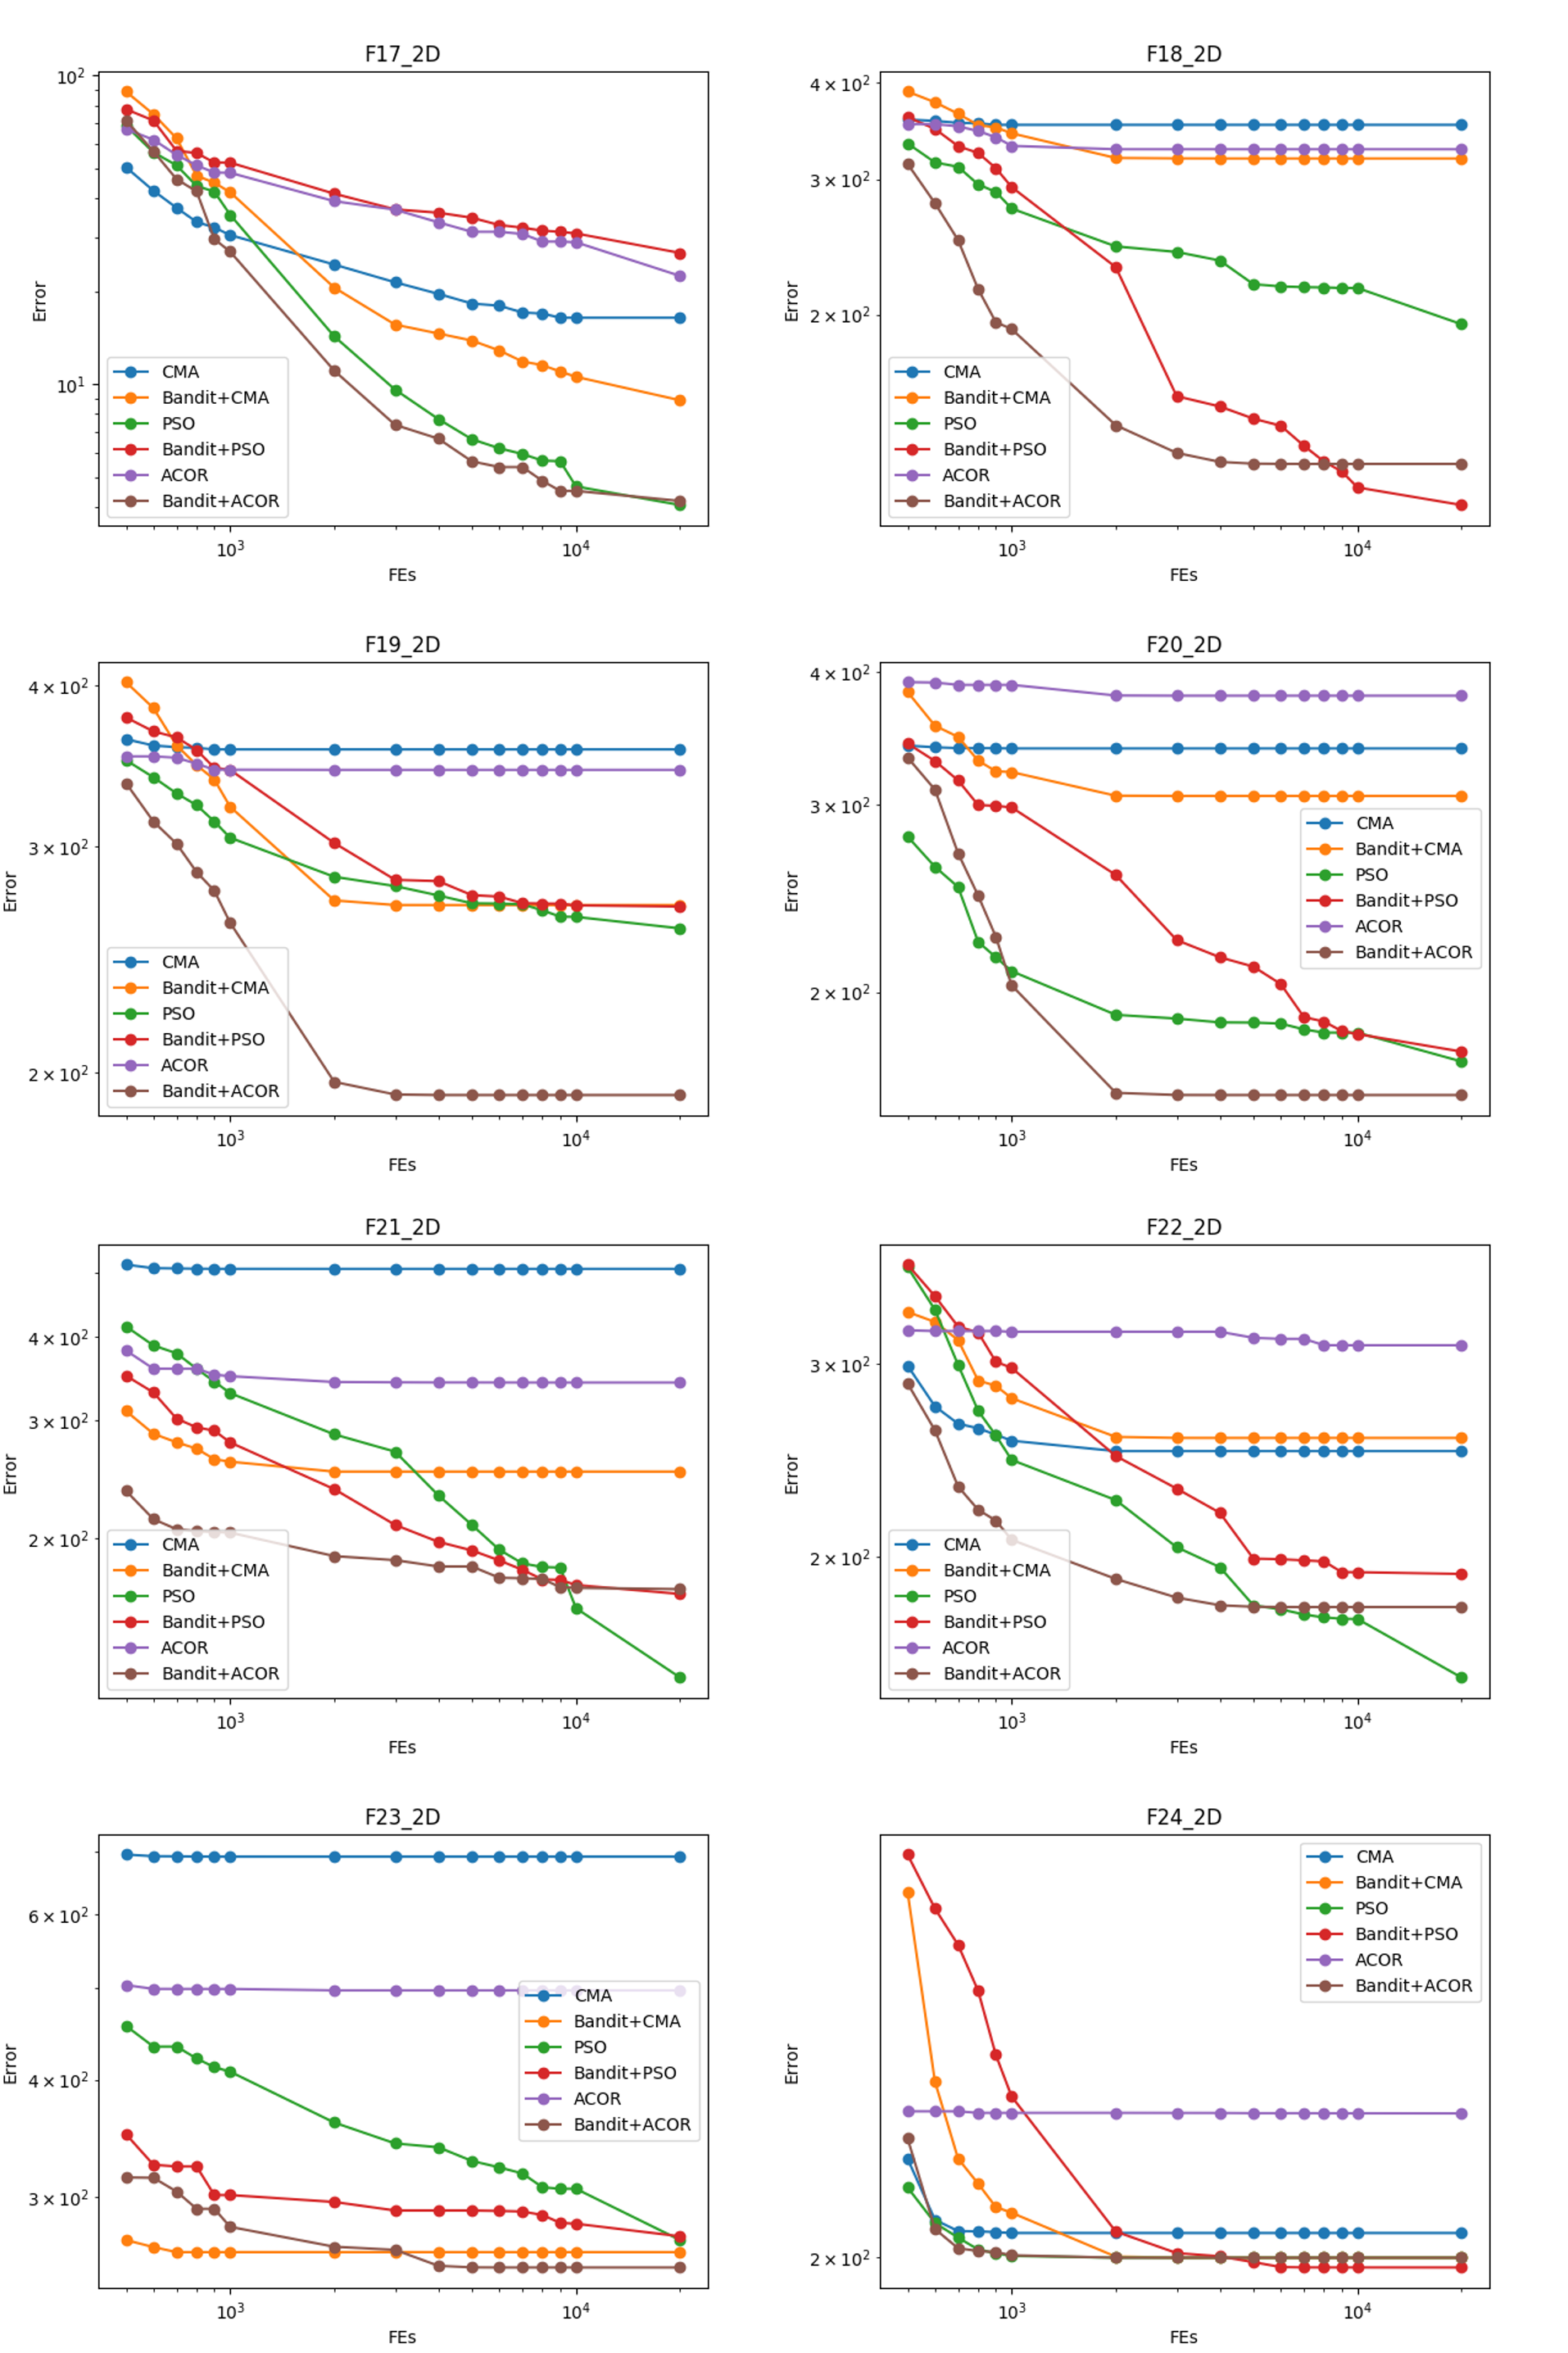
\includegraphics[width=\textwidth]{Average_F17_F24}
\caption{Average error of Problem 17 to Problem 24.}\label{fig:Average_F17_F24}
\end{figure}

\begin{figure}
\centering
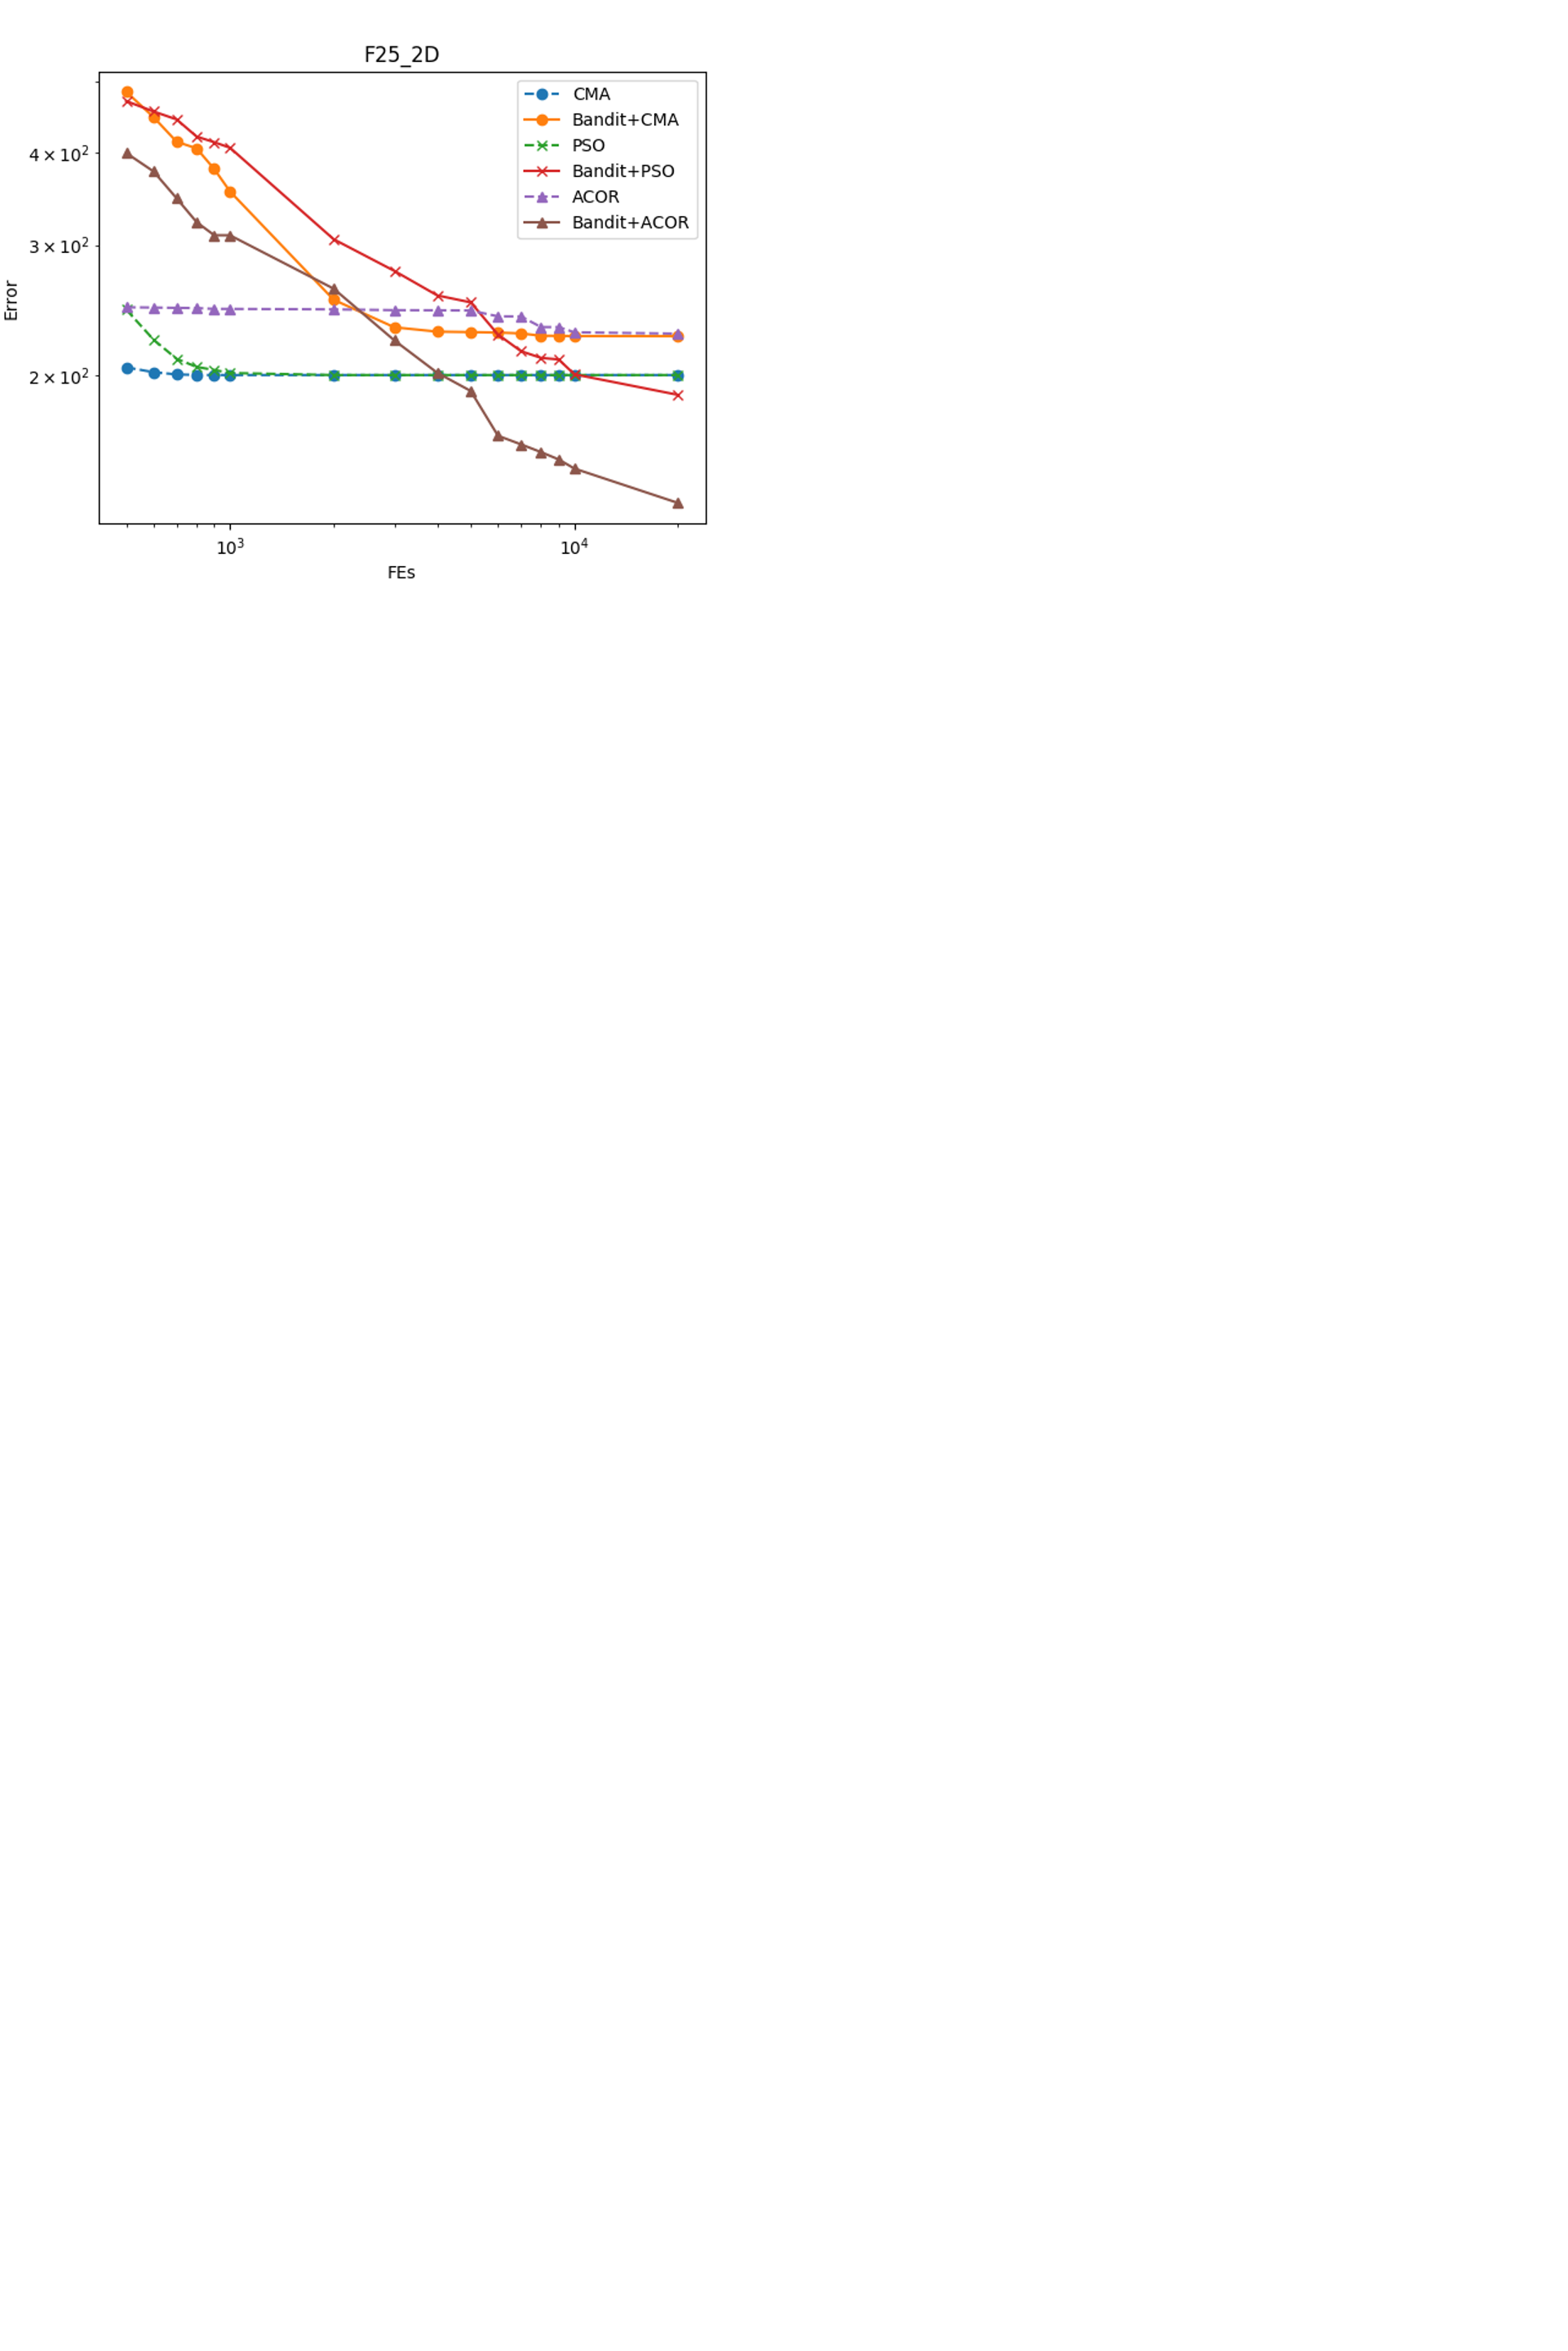
\includegraphics[width=\textwidth]{Average_F25}
\caption{Average error of Problem 25.}\label{fig:Average_F25}
\end{figure}

\begin{figure}
\centering
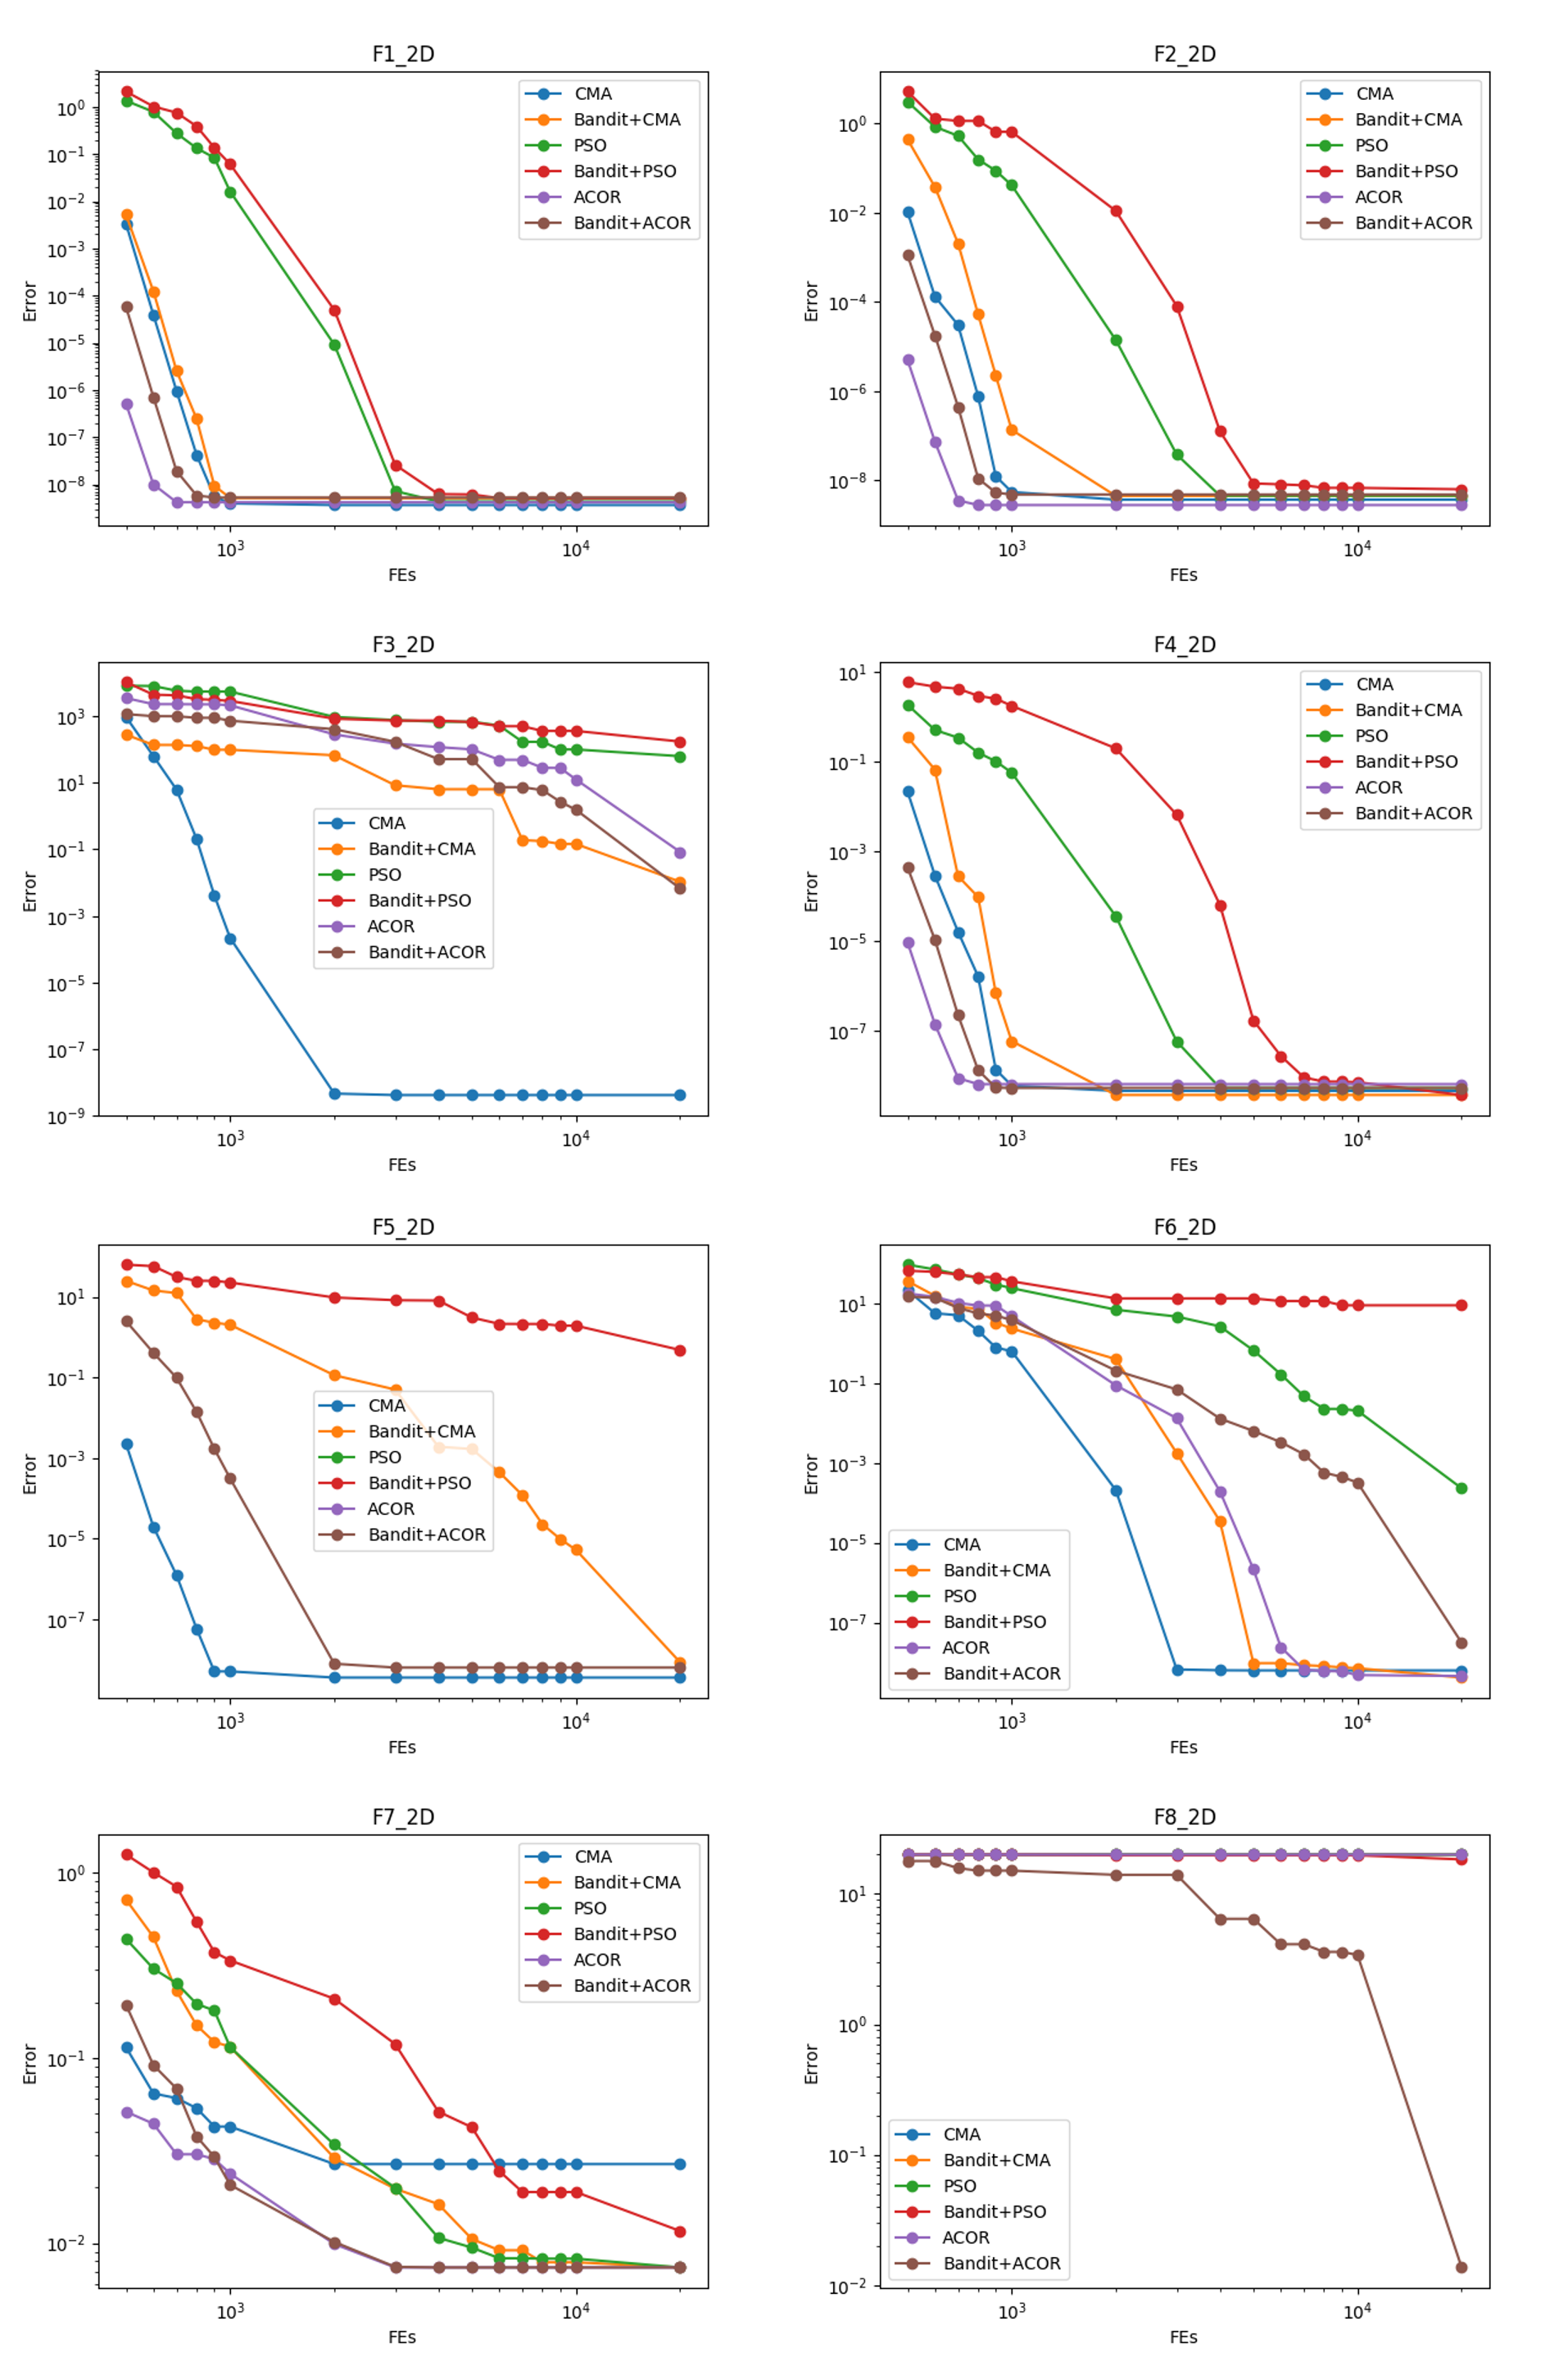
\includegraphics[width=\textwidth]{Median_F1_F8}
\caption{Median error of Problem 1 to Problem 8.}\label{fig:Median_F1_F8}
\end{figure}

\begin{figure}
\centering
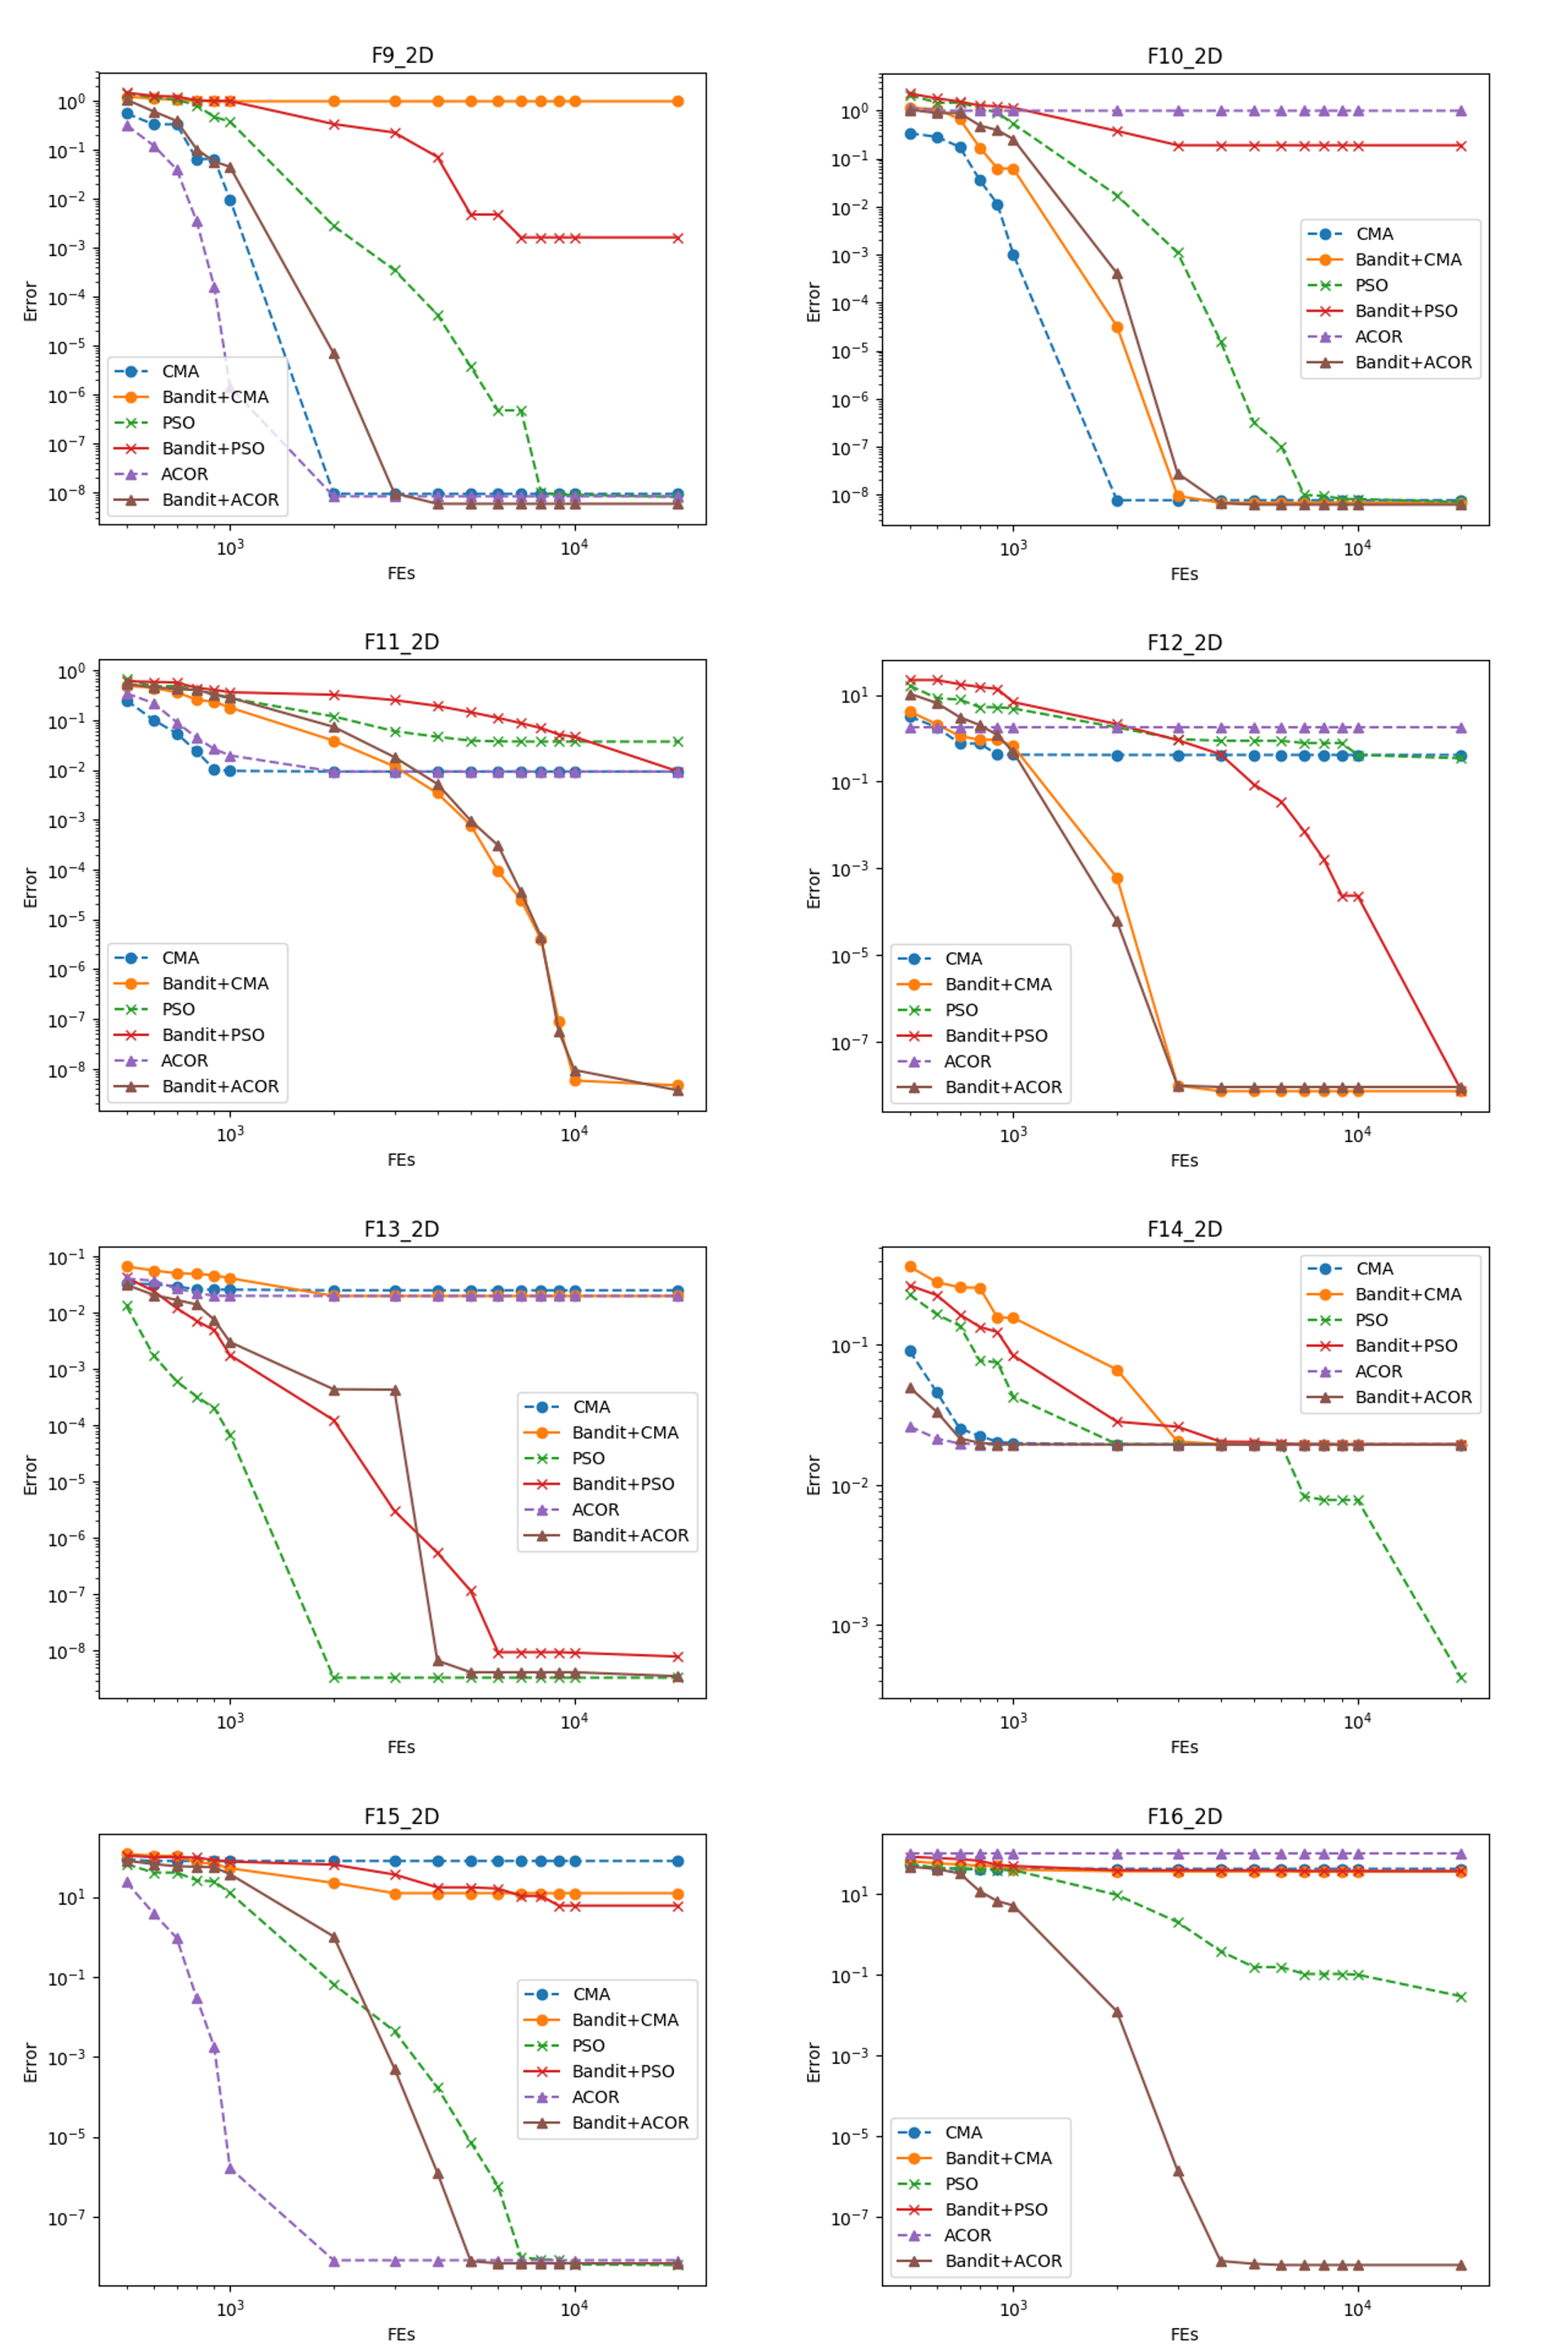
\includegraphics[width=\textwidth]{Median_F9_F16}
\caption{Median error of Problem 9 to Problem 16.}\label{fig:Median_F9_F16}
\end{figure}

\begin{figure}
\centering
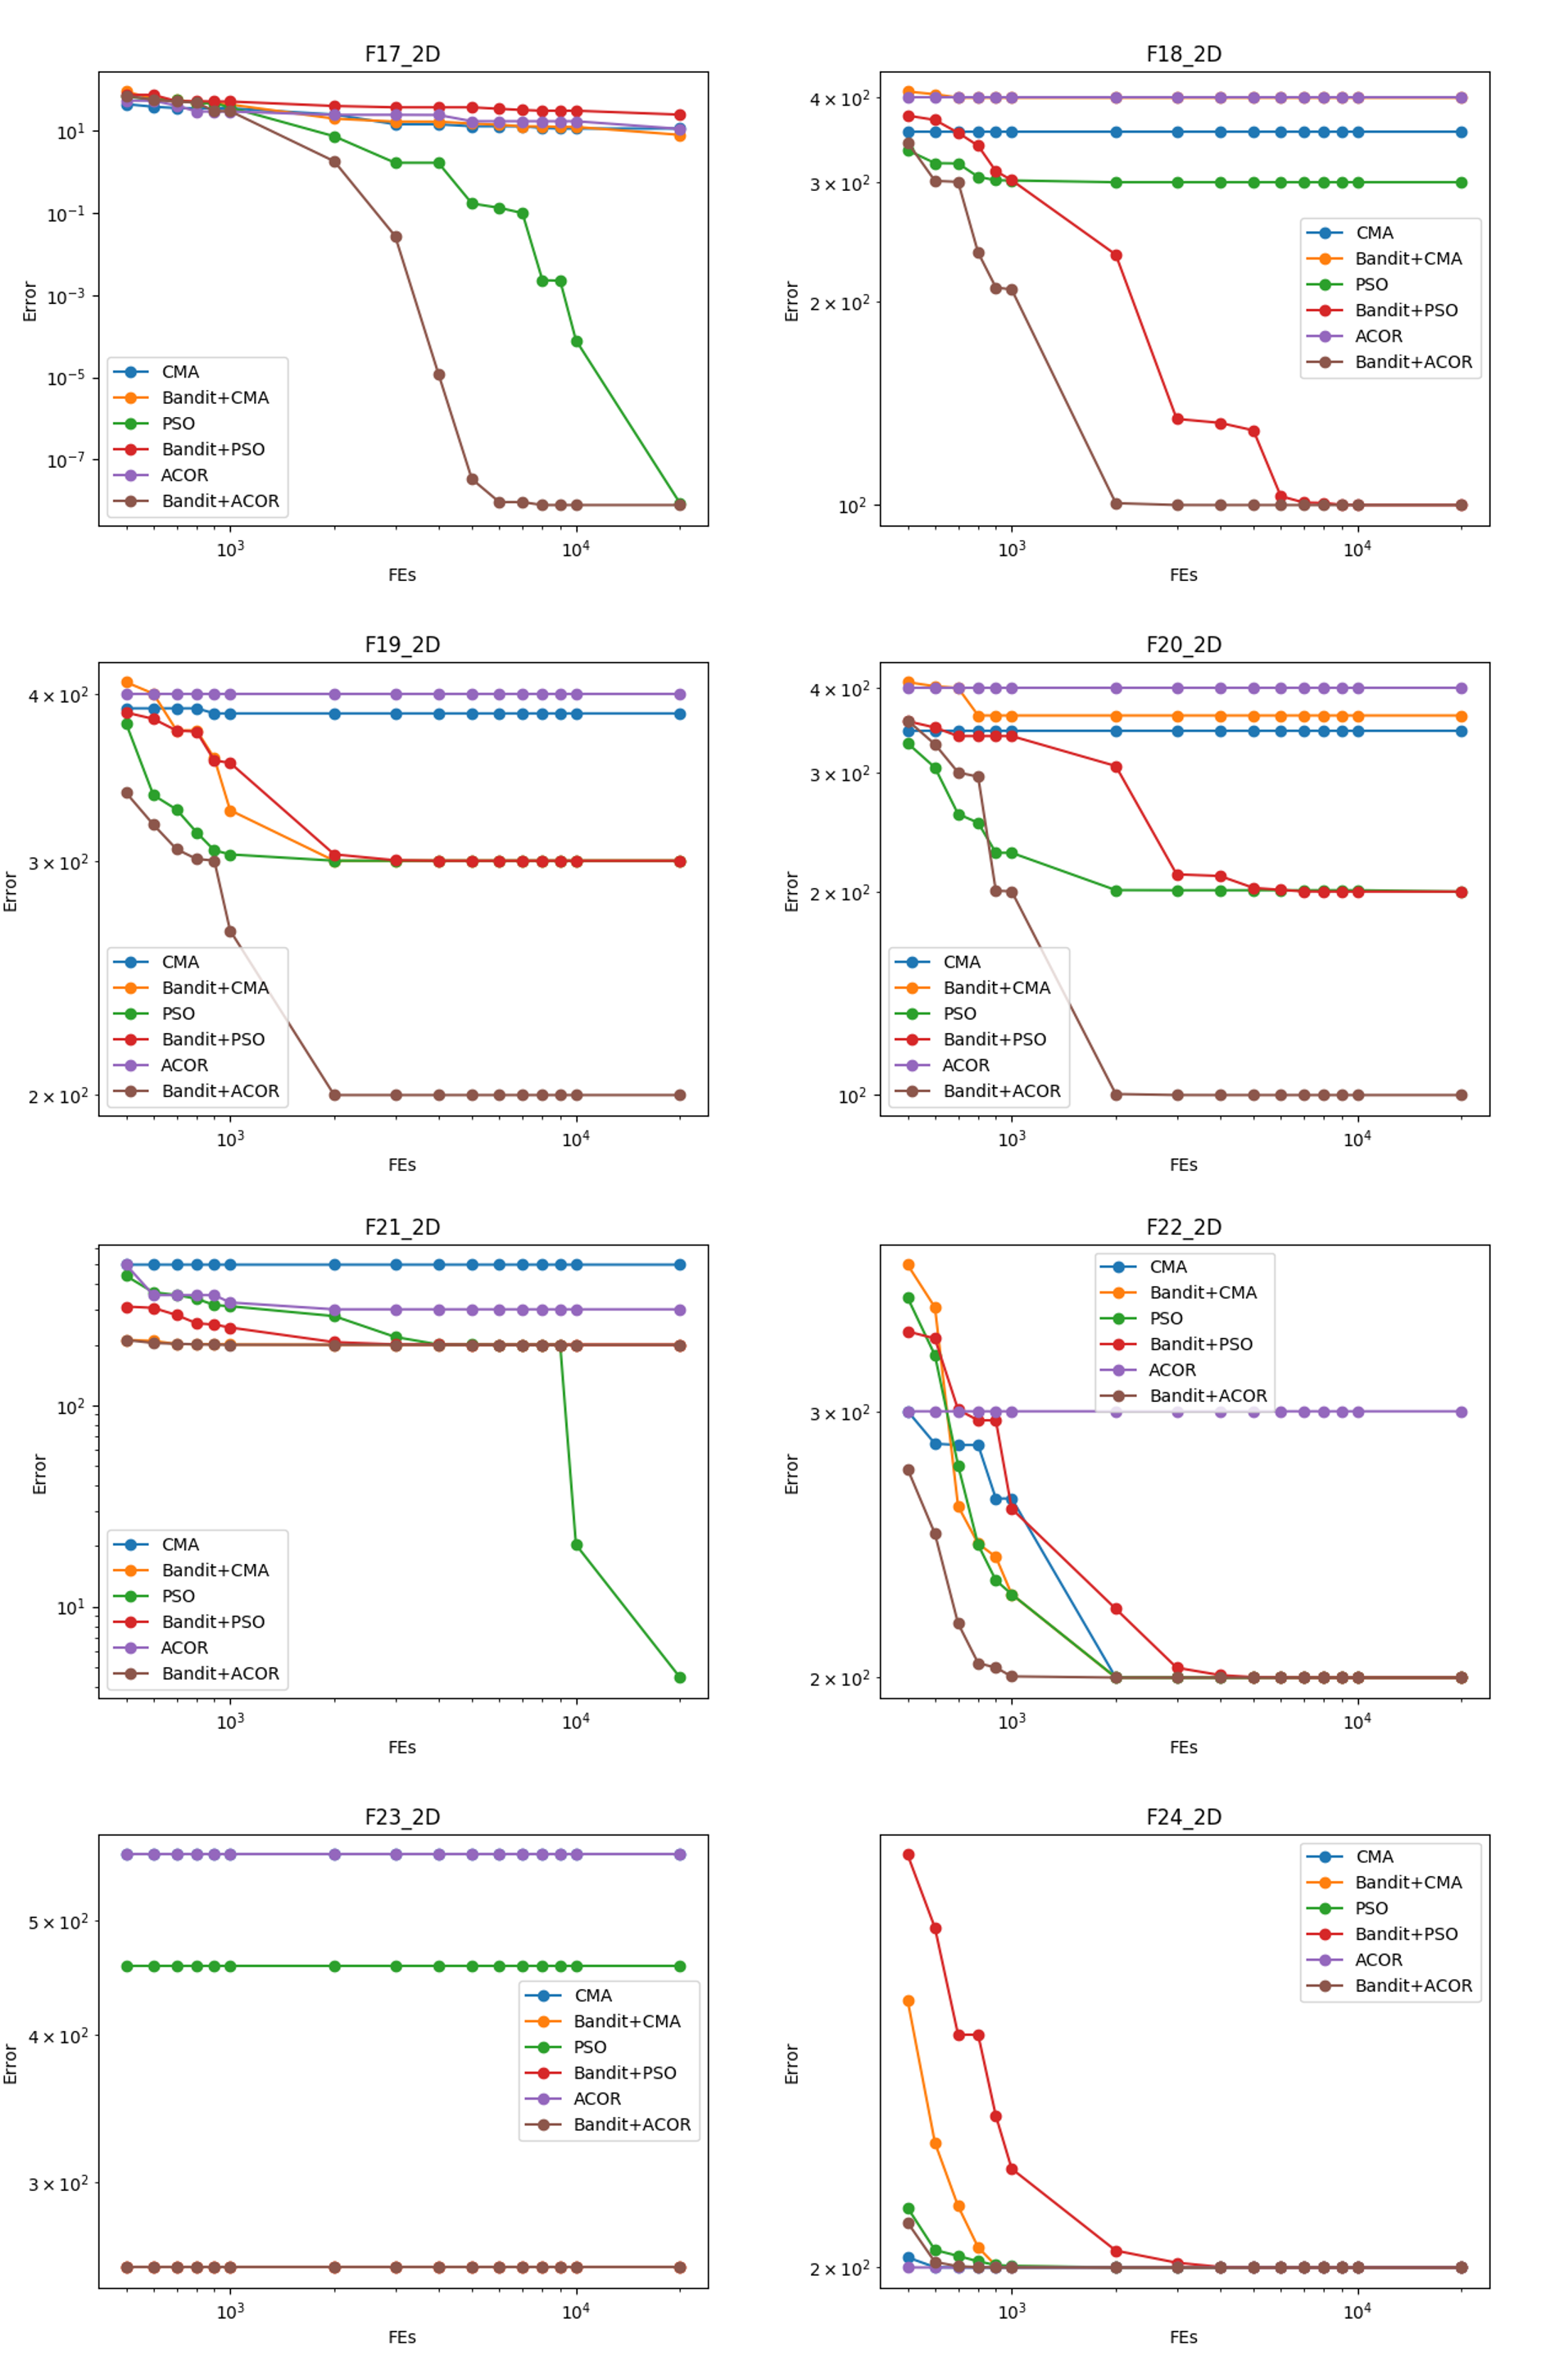
\includegraphics[width=\textwidth]{Median_F17_F24}
\caption{Median error of Problem 17 to Problem 24.}\label{fig:Median_F17_F24}
\end{figure}

\begin{figure}
\centering
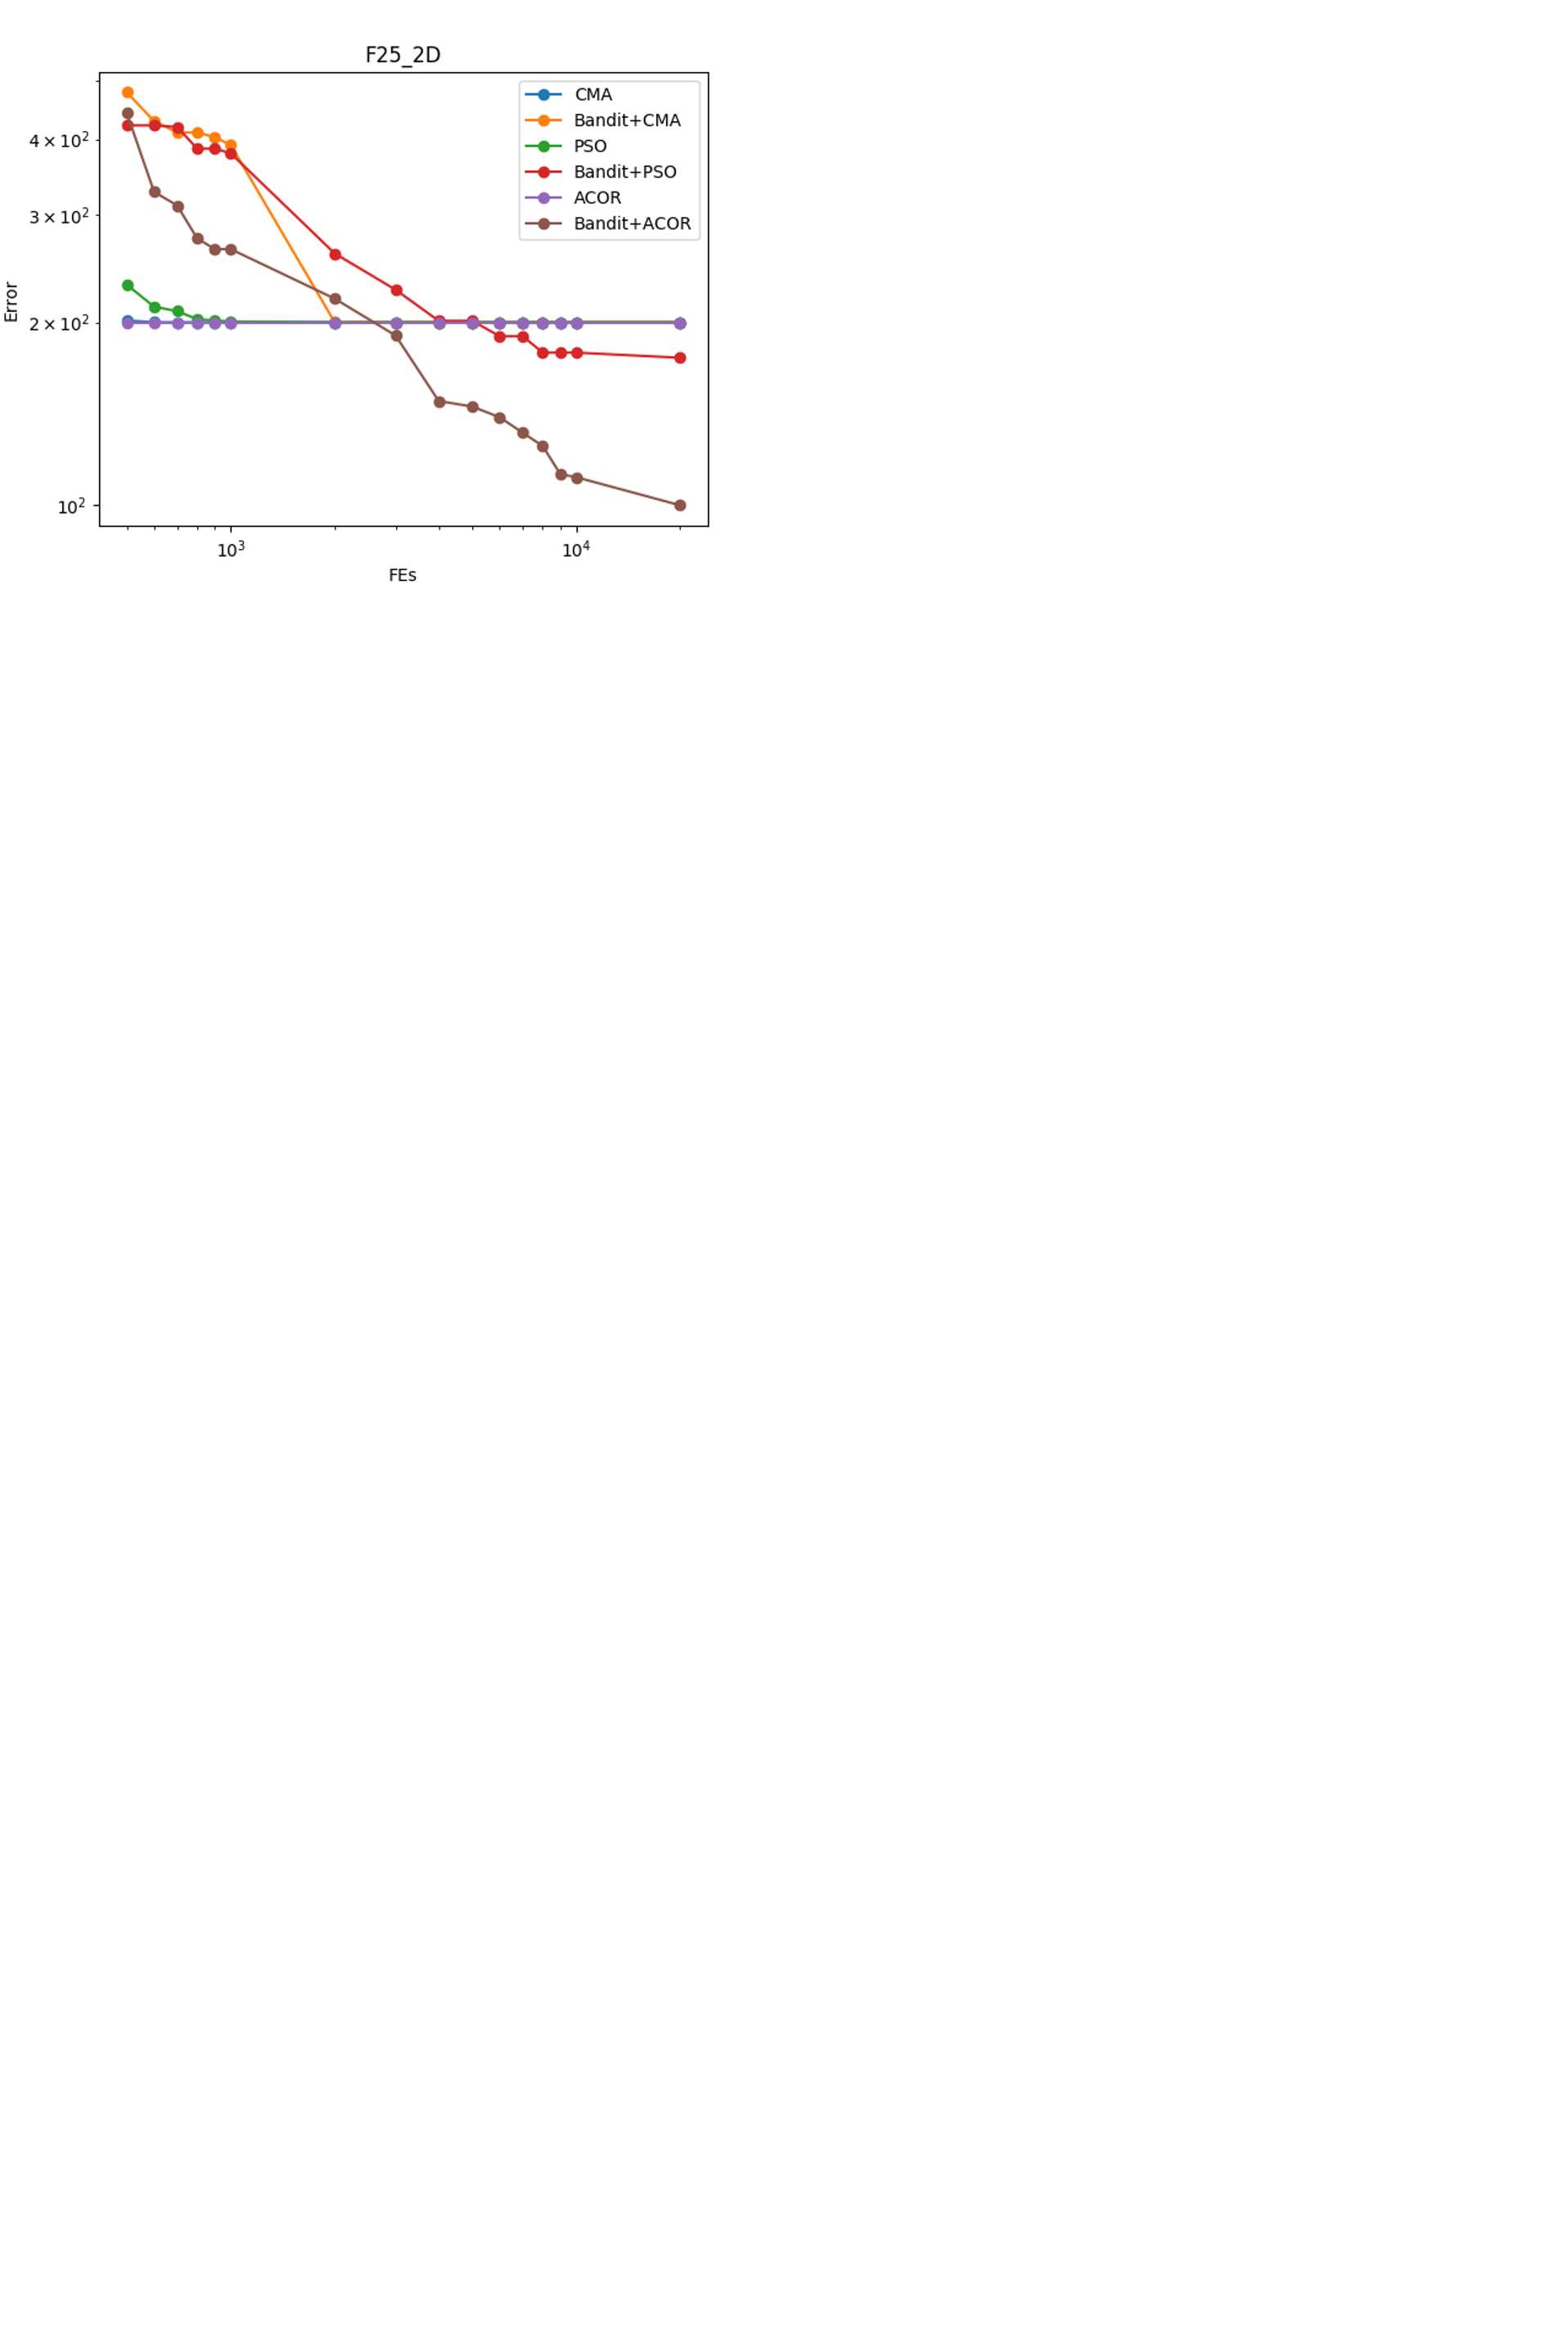
\includegraphics[width=\textwidth]{Median_F25}
\caption{Median error of Problem 25.}\label{fig:Median_F25}
\end{figure}

